% i will have better ideas in the future 
\documentclass[10pt]{article}
\usepackage[margin=0.5in]{geometry}
\usepackage{fontspec}
\usepackage{xcolor}
\usepackage{listings}
\usepackage{multicol}
\usepackage{parskip}
\usepackage{graphicx}
\usepackage{fontawesome5}
\usepackage{amssymb}

% Font setup
\setmainfont{DejaVu Sans}
\newfontfamily\titlefont{DejaVu Sans Bold}
\newfontfamily\codefont{DejaVu Sans Mono}[Scale=0.85]

% Colors
\definecolor{blueheader}{RGB}{90, 144, 160}
\definecolor{mygreen}{HTML}{65BA08}
\definecolor{codebg}{HTML}{DDCCCC}
\definecolor{codeframe}{RGB}{200, 200, 200}
\definecolor{lightgray}{HTML}{CACAFE}

% Listings style
\lstset{
    basicstyle=\codefont,
    backgroundcolor=\color{codebg},
    frame=single,
    framerule=0pt,
    framesep=3pt,
    rulecolor=\color{codeframe},
    breaklines=true,
    postbreak=\mbox{\textcolor{red}{$\hookrightarrow$}\space},
    aboveskip=5pt,
    belowskip=5pt
}

\begin{document}
\pagestyle{empty}

% Title
\begin{center}
  
\includegraphics[height=1.2cm]{zsh.png}
  \hspace{1em}
  {\titlefont\large \color{mygreen}Oh My Zsh Cheat Sheet}
  \hspace{1em}
  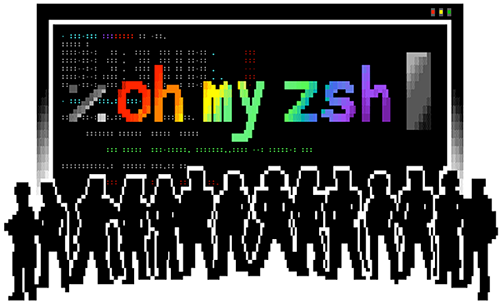
\includegraphics[height=1.2cm]{zsh2.png}

  \vspace{0.3em}
  \textcolor{lightgray}{\rule{\linewidth}{0.5pt}}
\end{center}

\vspace{0.5em}

\setlength{\columnsep}{20pt}
\begin{multicols}{2}

% Left Column (Networking)
{\titlefont\color{blueheader}\faNetworkWired\quad Key bindings }\vspace{5pt}

\textbf{\color{blueheader}Install oh-my-zsh}
\begin{lstlisting}
sh -c "$(curl -fsSL https://raw.githubusercontent.com/ohmyzsh/ohmyzsh/master/tools/install.sh)"
\end{lstlisting}

  \textbf{\color{blueheader}Walk}
\begin{lstlisting}
cd -         # move back to previous directory
[Ctrl] + [A] # move home
[Ctrl] + [E] # End of Line 
[Ctrl] + [F] # Forward by word 
[Ctrl] + [B] # Back by word  
\end{lstlisting}

\textbf{\color{blueheader} Edit}
\begin{lstlisting}
[Ctrl] + [U] # Clear to beginning of line 
[Ctrl] + [K] # Kill to end of line
[Ctrl] + [@] # Set Mark
[Ctrl] + [_] # Undo
\end{lstlisting}

\textbf{\color{blueheader}History}
\begin{lstlisting}
[Ctrl] + [R] # Search 
[Ctrl] + [P] # Match word on line  
\end{lstlisting}

\vfill\null\columnbreak

% Right Column (System and Tools)
  {\titlefont\color{blueheader}\faTools\quad Commands && Globs}\vspace{5pt}

\textbf{\color{blueheader}Commands}
\begin{lstlisting}
fg  -> Restore process from suspend
bg  -> Continue process in background  
!!  -> Last command 
!*  -> Last command's parameters 
!^  -> Last command's first parameter 
!$  -> Last command's last parameter 
\end{lstlisting}

\textbf{\color{blueheader}Basic}
\begin{lstlisting}
?         -> Any char
*         -> Any string 
[class]   -> Any single class
[^class]  -> NOT from class -> use Regex 
(foo|bar) -> alternative
**        -> recursive dirs 
***       -> recursive dirs and symlinks 
\end{lstlisting}

\textbf{\color{blueheader}Entries}
\begin{lstlisting}
*(.)      -> match file 
*(/)      -> match dir
*(@)      -> match symlink
\end{lstlisting}

\end{multicols}
\end{document}
